\section{Anpassung}
Die Übung dient dem Studierenden sich mit der Laborausrüstung und Messtechnik in der Mikrowellentechnik vertraut zu machen. Als Messobjekte dienen einfache Schaltungen mit Mikrostreifenleiter, welche mit Kupferband selber hergestellt wurden.
\subsection{Ziel}
\subsection{Messungen}
\subsubsection{Dämpfungsmessung einer Mikrostreifenleitung}
Eine Mikrostreifenleitung von 50 Ohm auf einer FR4 Leiterplatte solle etwa 3 mm Breit sein.
Parameter:\\
\begin{itemize}
\item $\epsilon_{r}$ von FR4 = 4.4
\item Dicke FR4 = h = 1.6mm
\item Höhe der Kupferschicht = T = $35 \mu m$
\end{itemize}
Zum Auslesen der Wellenimpedanz aus der Grafik wird das Verhältnis von $\frac{W}{h}$ benötigt.

Ist die  Impedanz bekannt, so kann nach die Formel $Z0=\dfrac{W}{h}$ nach h umgestellt werden und h mit Hilfe der Grafik in Abbildung \ref{Z0_Grafik} bestimmt werden.
\begin{figure}[htbp]
	\centering
		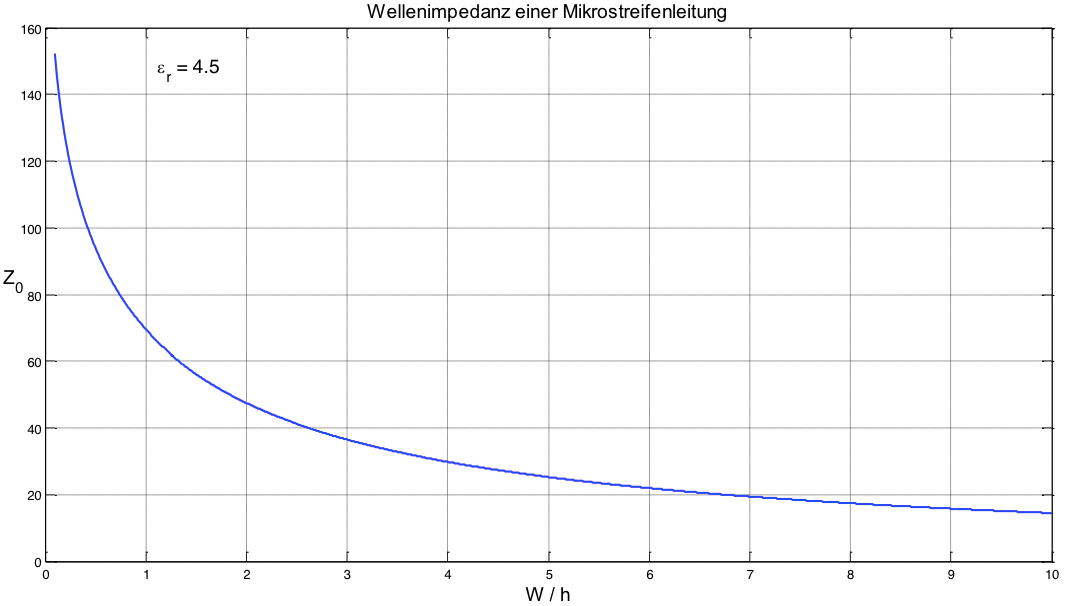
\includegraphics[width=8cm]{content/Bilder/Z0_Grafik.png}
	\caption{Wellenimpdedanz Z0}%
	\label{Z0_Grafik}
\end{figure}

Die Breite des Mikrostreifenleiters kann auch berechnet werden.
\[Z0=\sqrt{\dfrac{\mu_{0}*\mu_{r}}{\epsilon_{0}*\epsilon_{r}}}*\frac{h}{W}*\left[1+1.735*\epsilon^{-0.0724}*\left(\dfrac{W}{h}\right)^{-0.836}\right] ^{-1}\]

Gerader Mikrostreifenleiter von der Breit 3 mm mit einer Impedanz von 50 Ohm auf einer FR4 Platte. Die Dämpfung kann mit einer $S_{21}$ Messung bestimmt werden.

\subsubsection{Reflexionen an einem 90$^\circ$ Winkel}
Eine 50$\Omega$ Leitung mit einem 90$^\circ$ Winkelverlauf ohne Gehrung auf einer FR4 Platte. Die eine Seite wird mit 50$\Omega$ abgeschlossen.
Die Reflexionen soll mit einer $S_{11} $Messung gemessen werden. Messfrequenz ist 1.5 GHz.

Auftrag:\\
Verbessere die Leitungsimpedanz, indem die Diskontinuität am  90$^\circ$ Winkel mit Hilfe einer Gehrung kompensiert wird. Messe dabei immer wieder die Reflexionen. Um wie viele dB konnten diese reduziert werden?


\subsubsection{Anpassung an eine Last RL 100 $\Omega$}
Die 50 $\Omega$ Leitung soll mit einem 100 $\Omega$ zur Masse  kurzgeschlossen werden. In der folgende Abbildung \ref{RL100} zeigt den Aufbau.

\begin{figure}[h!]
	\centering
		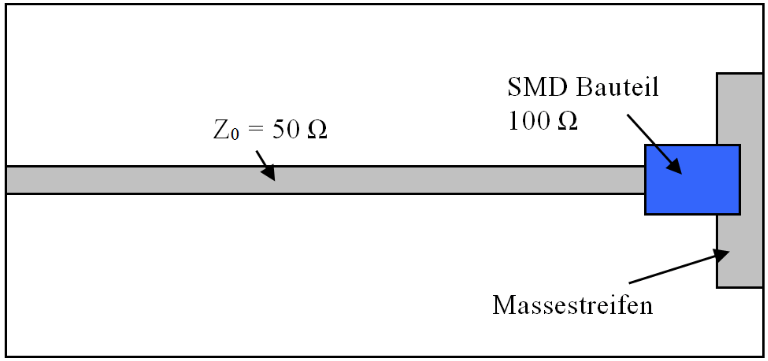
\includegraphics[width=8cm]{content/Bilder/50OhmLeitungRL100.png}
	\caption{50 Ohm Leitung mit RL100}%
	\label{RL100}
\end{figure}

Auftrag:\\
Die Reflexion $S_{11} $am Eingang der Leitung für einen Frequenzbereich von 1 bis 2 GHz. \\
Welche Reflexion würde man direkt beim Widerstand erwarten? \\
Realisiere eine Anpassung für eine Entwurfsfrequenz von 1.6 GHz mit Hilfe einer offenen, parallelen Stichleitung. Welcher Wert für $S_{11} $wird am Eingang erreicht? Mindestens $-20$ dB sollten schon erreicht werden 